% methods.tex -- \section{Method} for the ICLR 2027 main file, after related_work.tex.
% v2, rewritten 2026-09-14 on the PI's instruction (design and the motivation behind each
% decision, intuitive mechanism, one figure of the mechanism), synthesised from three
% drafts (teacher, reviewer-proof, designer) by the graft list of the same date. Facts,
% source comments and the instrument table are carried from the 2026-09-12 revision; the
% prose is new and is written around Figure 1 (figures/fig_mechanism_{a,b,c}.pdf, panels
% A embodiment, B the collective, C the flag). Review of 2026-09-14 applied (fire-rate
% estimator over all debates in the two-by-two readouts, the other party's stake, the
% weighted-majority clause made analytic, controls held at the registered protocol rather
% than byte-identical, the writer's one forbidden assertion, 16.17 replays only r0 to r2,
% line pointers, cell rule populations, the record's reasons for a stated change, parse gate
% over the embodied baseline, figure fallback re-laid so A and C are legible). Every number
% carries a LaTeX comment naming its source: prereg = Guidance_Documents/prereg_embodiment_community.md, code = scripts/*.py,
% artefact = divergence_study_outputs/*, design = papers/embodied_sensor/graph_theory_design.md
% (section number).
% Prereg sources: L3-4, L34-37, L42-56, L75-76, L105-107, L139, L227-238, L296-303,
%   L396-397, L528-542, L594-595, L755-770, L1169-1181, L1240-1252, L1297-1301, L1307-1310,
%   L2285-2340, L2366-2373, L2492-2497, L2566-2589, L2594 (Dilemmas fire rate, silence),
%   L3044-3069 (16.1 check 1, composite against the stake-blind counter), L3251-3277, L3292,
%   L3300-3318, L3335-3340, L3504-3570 (16.10 registration), L3584-3594 (16.11a registration),
%   L3608-3612 (16.11a RESULTS), L3639-3651, L3653 (16.12 flooding), L3664-3666 (16.12 table,
%   the flag's defining rates), L3704-3786 (16.14 registration), L3817-3833 (16.14 RESULTS,
%   guard facts only), L3871-3886 (16.14b registration), L3888-3999 (16.15 registration),
%   L4091-4097 (16.14b RESULTS, guard facts only), L4136-4142 (16.10 RESULTS, guard facts
%   only), L4160 (16.10 RESULTS, per-seat opening rates, the two lock numbers), L4212-4259
%   (16.15 estimator and frame), L4263-4268, L4275 (16.15.1 RESULTS, lift and ratio columns,
%   definitions only), L4285-4326, L4462-4470, L4494-4496 (16.15.4 RESULTS, majority equals
%   the neutral seat on 1,642 of 1,642, best seat neutral, motivation only), L4515-4529;
%   L4034-4048 (16.13 instrument), L4719-4791, L4753 (binding games, silence), L4793-4870,
%   L5018-5058, L5060-5106, L5108-5145, L5147-5192, L5114-5117 and L5129-5131 (coordination
%   scoring rule); L5194-5215 (16.16 registration), L5251 and L5261-5269 (16.16 RESULTS,
%   per-seat opening rates and the pre-declared reading), L5309-5345 (16.17 registration),
%   L5539-5580 (16.18 registration), L5720-5750 (16.19 registration), L6100-6150 and
%   L6183-6184 (16.21 registration).
% Design-document sources: graph_theory_design.md sections 1, 2(a)-(g), 3, 6.
% Code sources: run_phase1_quartet.py:77-116; run_stance_factorial.py:189-199,362-396,438-441;
%   run_bm_embodiment.py:60-67,83-104,138-155; run_bm_cross_sig.py:72-86;
%   run_crowdgold_aita.py:197-230,417-427,972-999; run_crowdgold_deliberation.py:12-28,
%     400-402,461-511,522-540,544-556,557-570,576-586,587-597,616-660,634-647,668-672,685-697,
%     720-751,753-770,786-818,820-885,889-904,1043-1046,1070,1180-1205,1227,1298,2092-2129,
%     3297-3317,3532-3538,3620-3623;
%   run_crowdgold_topology.py:45-61,86-127; run_crowdgold_unembodied.py:97-160,179-200;
%   run_crowdgold_dilemma.py:121-136,229-312; run_bm_cycle.py:78-136,228-258;
%   run_crowdgold_modvendor.py; run_crowdgold_multivendor.py; run_crowdgold_coalition.py;
%   run_crowdgold_nperspective.py; screen_third_party.py;
%   load_scruples.py:10-13,128-132,356-359,771-786; load_scruples_dilemmas.py:16-27;
%   load_brokenmath.py:4-5; verdict_format.py:32-34,100-101,263-280,380-449; generators.py:624;
%   analyze_bm_embodiment.py:27-31,70-97; analyze_crowdgold_sdt.py:113-131;
%   analyze_loop_step.py:88-111,205-214; analyze_claim_audit.py:60-107;
%   analyze_stake_grip.py:39,57-68,151-179; analyze_unembodied_ablation.py:68-70,88-117,144-215,275-276;
%   analyze_topology_2x2.py:18-19,129-130,141-157,184-204,227,339; analyze_actuator_ladder.py:53-64,103-104,152-175;
%   analyze_dilemma_grip.py:62-66; analyze_dilemma_sensor_search.py:111-116;
%   analyze_router_decomposition.py:97-101,139-168,183-247,251-263,322-347,374-448;
%   analyze_effective_voter.py:21-31,106,177-247; analyze_bm_notes.py; analyze_length_matched_elephant.py;
%   elephant_scorers.py:20-48,165-193; rescore_elephant_untruncated.py:1-30,65,112,122-164;
%   run_elephant.py:376; tmg_games.py; run_game_singleagent.py; analyze_game_coordination.py.
% Artefacts: crowdgold_aita_summary.json:6-11 (+wrapper_match); cg_delib_pilot_console.log:2,40;
%   length_matched_elephant_oeq_validation_corrected.json; router_decomposition.json;
%   effective_voter.json; transfer_readouts.json; topology_2x2_analysis.json; bm_cycleb_analysis.json;
%   emergent_graphs.json (protocol.nodes, protocol.stages, protocol.edges, one_loser_firings_split);
%   game_solo_analysis.json; game_solo_masked_analysis.json; game_B1_analysis.json;
%   game_B2_analysis.json; game_C1_analysis.json; game_solo_nb_analysis.json;
%   game_coordination_analysis.json.
% Style matches introduction_clean.tex: no em dashes, no colons or semicolons in running
% prose, no lists in prose, past tense for what was done, present tense for what holds.
% Terminology as abstract_clean.tex and introduction_clean.tex: seat, brief, side, stake,
% moderator, verdict, objection, flag, the collective, narration as the light dose.
% Results are NOT stated here beyond the two lock numbers (99.7 / 97.4), the flag's
% defining rates (92 / 7 on one-loser verdicts) and the 16.16 amplifier reading the PI
% asked for; every other readout is in results.tex.
% Cites milgrom1986relying, dewatripont1999advocates, krishna2001model, lipman1995robust,
% golub2010naive, mercier2011argumentative, longino1990science, shapley1984optimizing,
% ladha1992condorcet, petrov2025brokenmath, cheng25elephant, openai_gpt54nano,
% anthropic_haiku45, anthropic_sonnet46, xai_grok41, all present in references.bib
% (grep 2026-09-14). Scruples (Lourie, Le Bras & Choi, AAAI 2021) has NO bib key; a \todo
% marks the spot and no key is invented.
% \todo requires the todonotes package or the fallback macro below.
% The main file needs \usepackage{booktabs} for the table and \usepackage{graphicx} for
% the figure; nothing else (no adjustbox). The old labels sec-method-interventions,
% sec-method-designs, sec-method-measures and sec-method-estimation are kept as aliases
% because comments in results.tex and introduction.tex name them.
% Prose budget 1,300-1,600 words (non-comment tokens outside the table and figure float,
% section, subsection, label, providecommand and todo commands dropped, citation tokens
% counted); this file counts 1,599 by that rule (scratchpad/count_methods.py) after the
% review edits; compiled with tectonic against the three panel PDFs and references.bib on
% 2026-09-14.

\providecommand{\todo}[1]{\textbf{[TODO: #1]}}

\section{Method}
\label{sec-method}

\begin{figure}[t]
\centering
% Figure 1, three Graphviz panels from make_mechanism_figure.py (fig_mechanism_{a,b,c}.pdf):
% A over C at the left, the portrait B at the right, so every panel is legible at column width.
\begin{minipage}[c]{0.57\linewidth}\centering
\textbf{A}\\[2pt]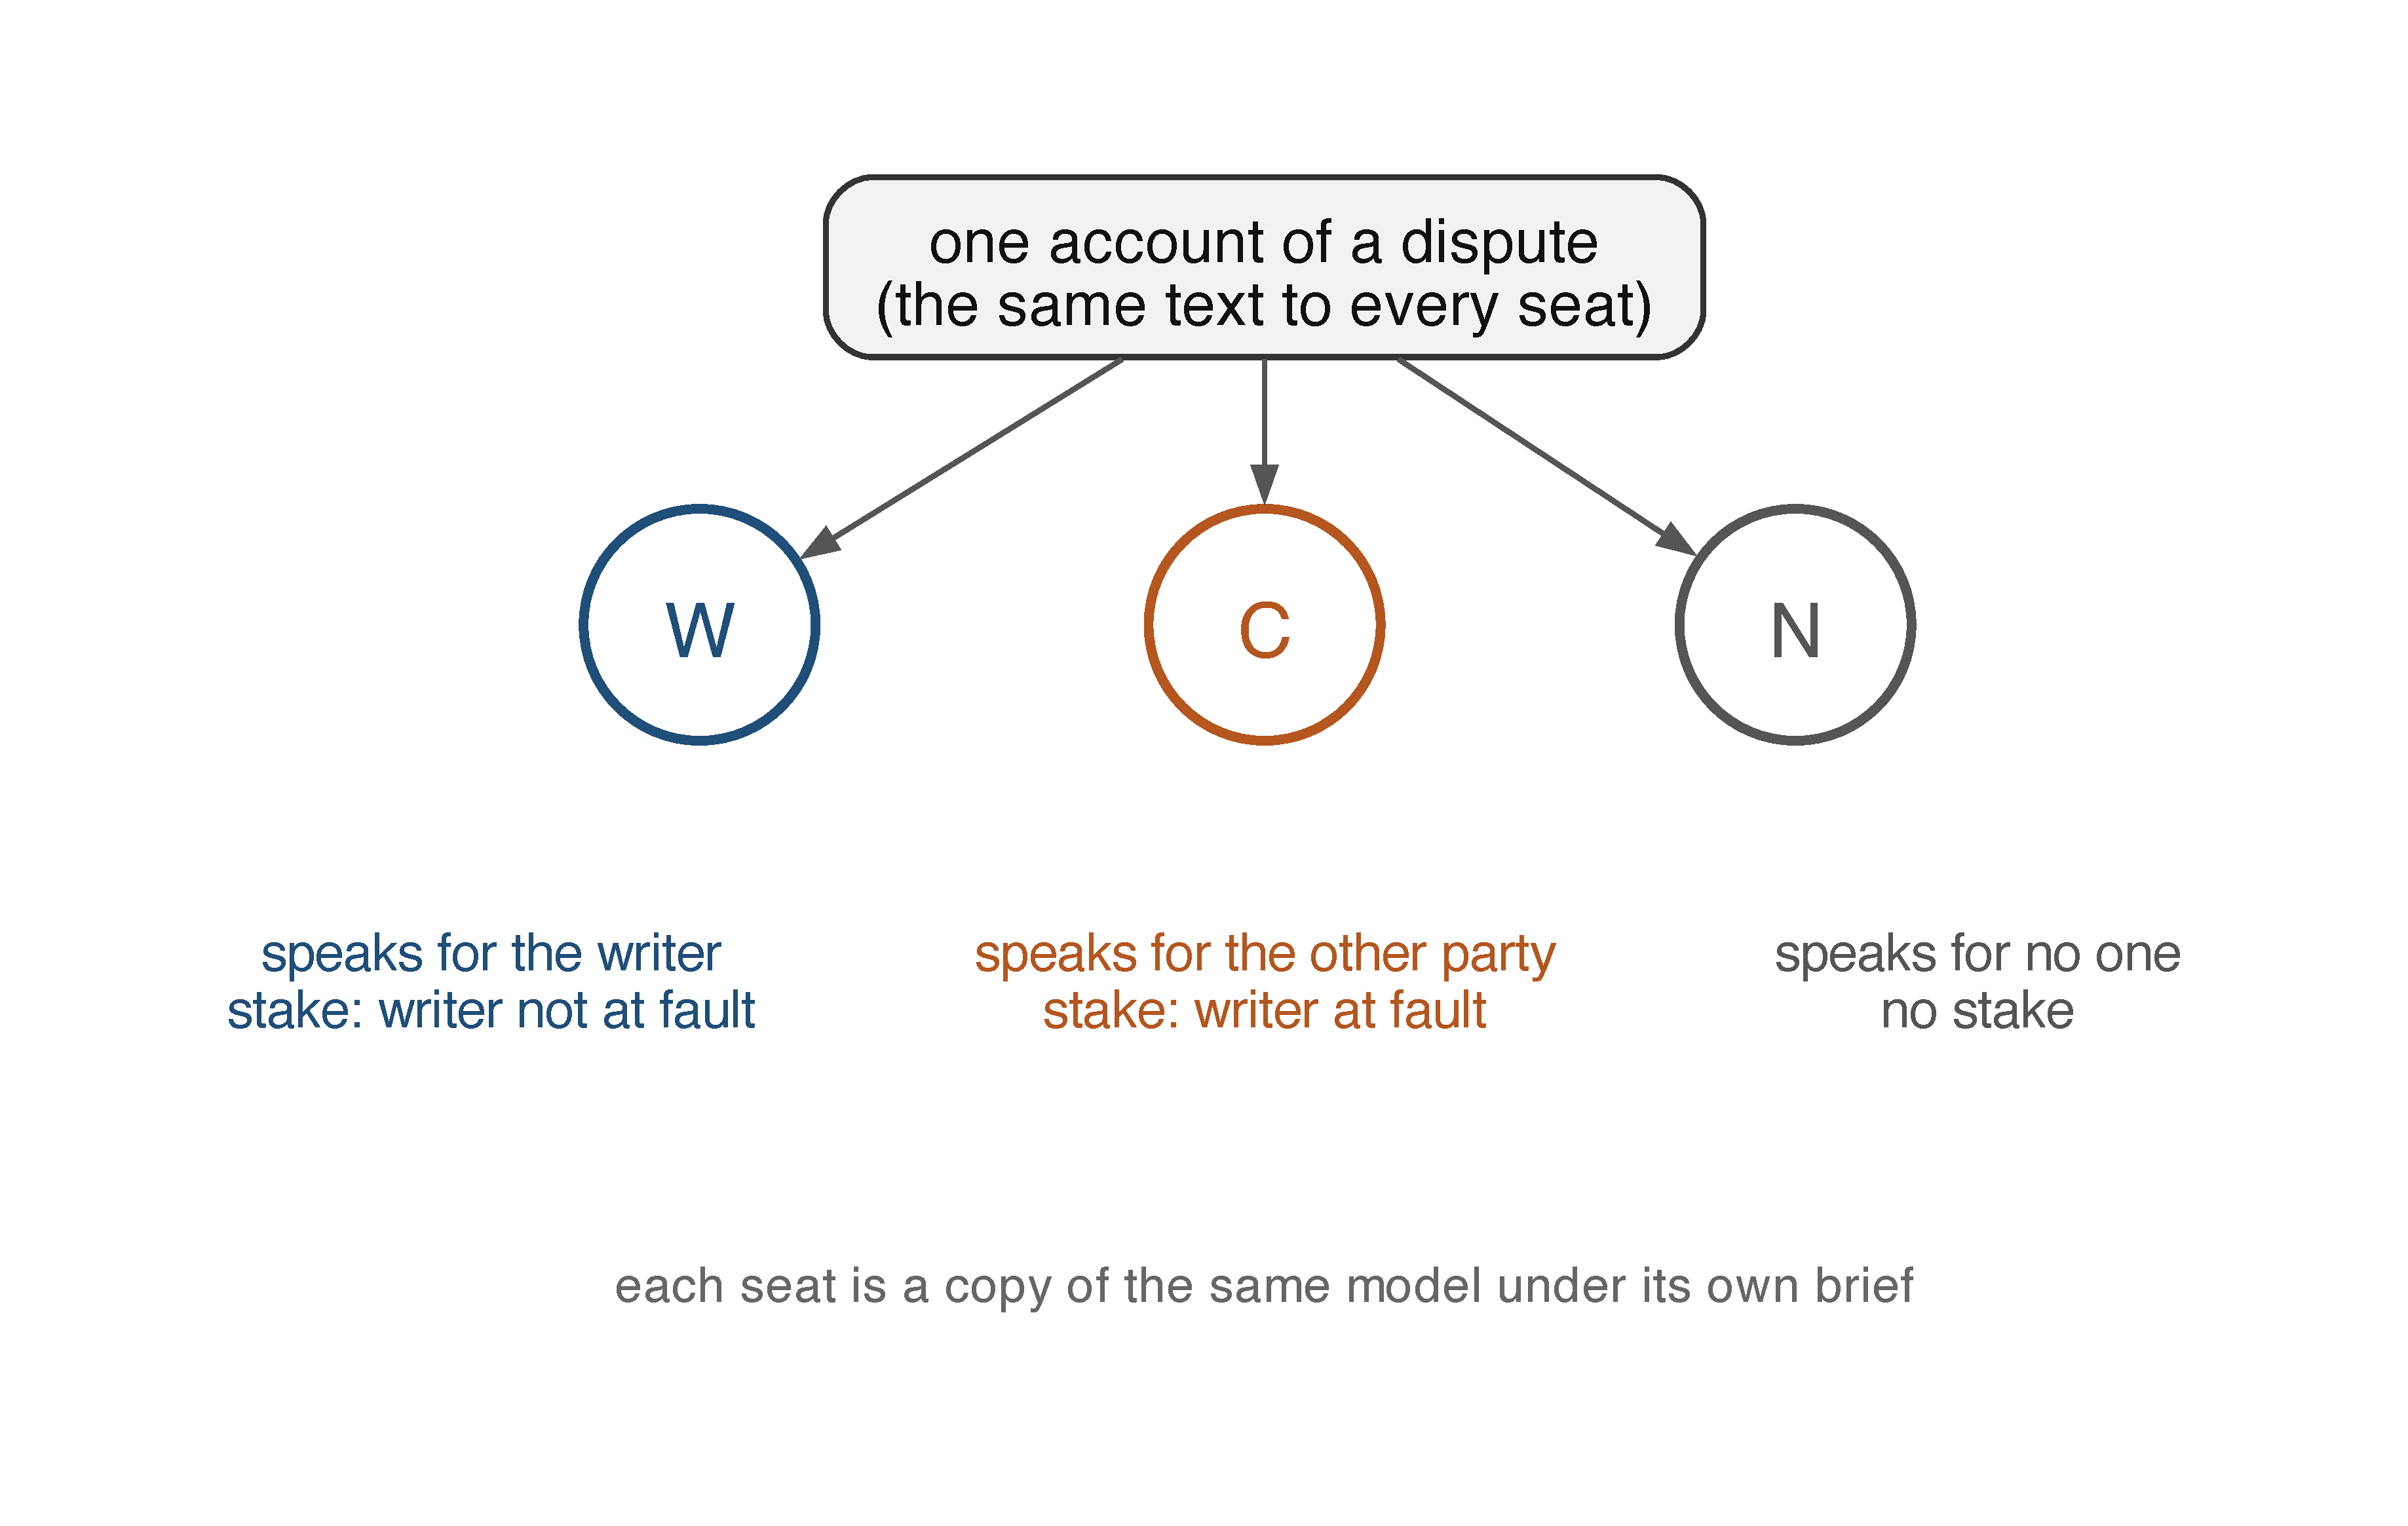
\includegraphics[width=\linewidth]{figures/fig_mechanism_a.pdf}\\[10pt]
\textbf{C}\\[2pt]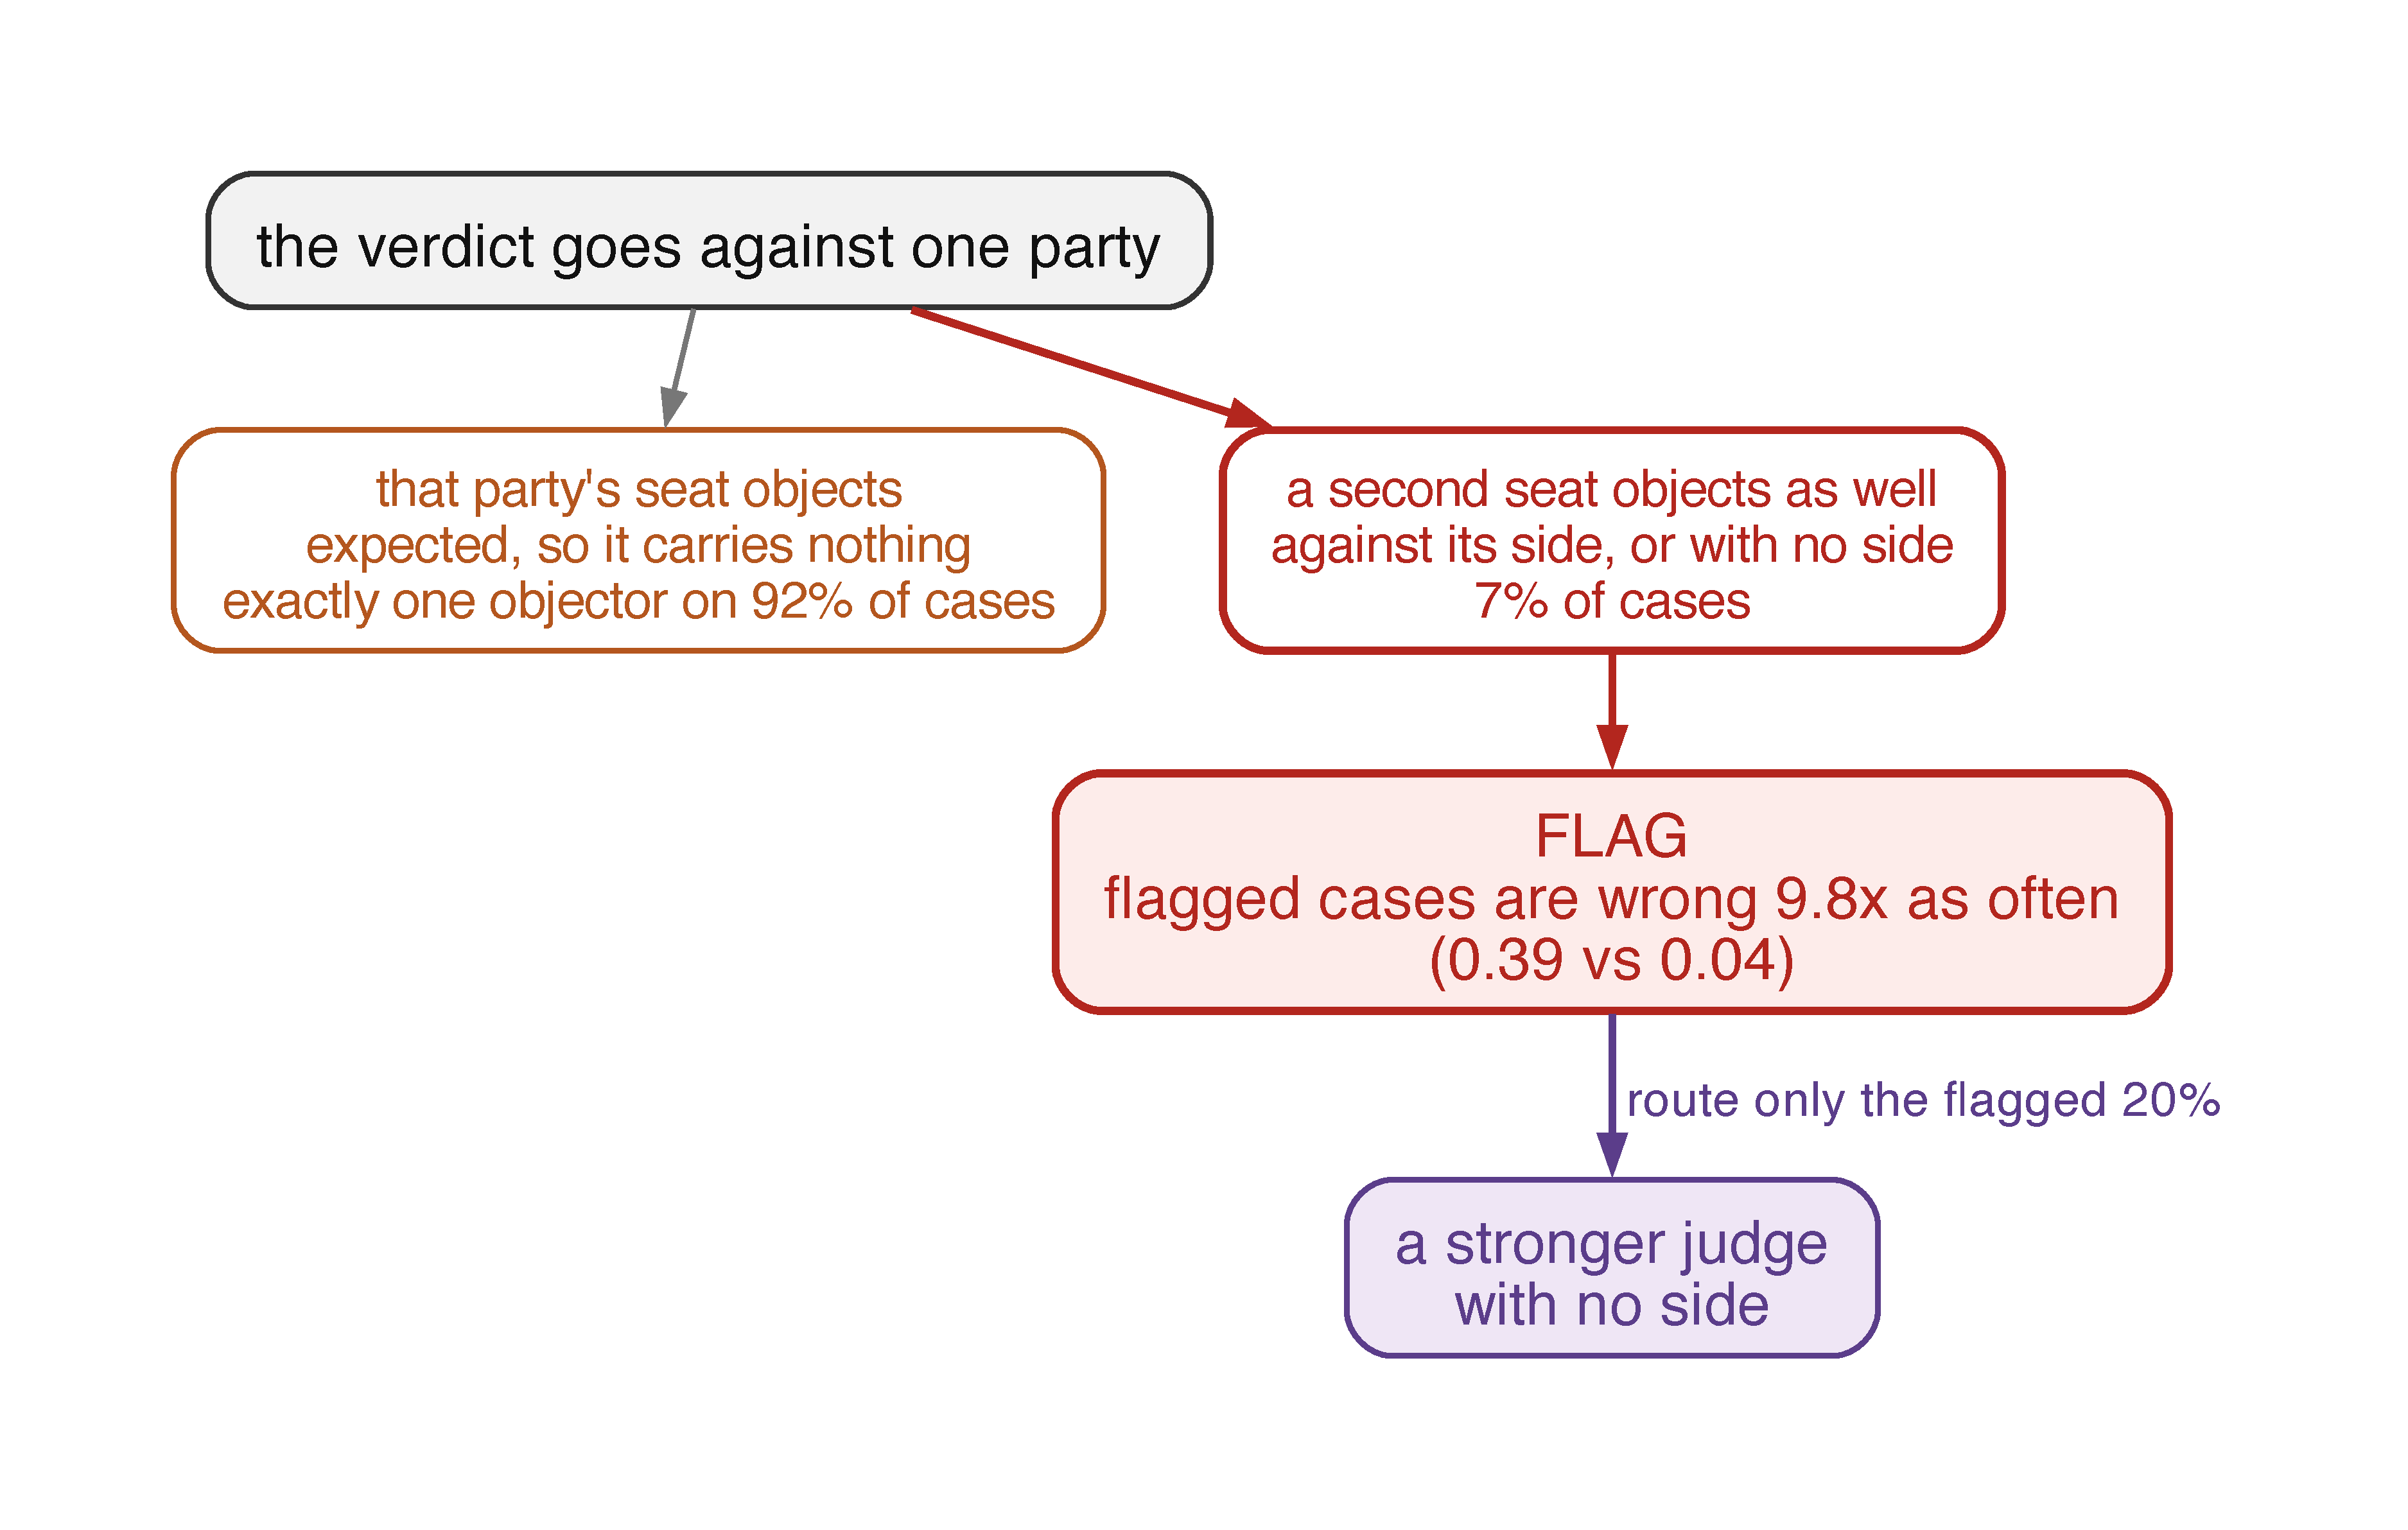
\includegraphics[width=\linewidth]{figures/fig_mechanism_c.pdf}%
\end{minipage}\hfill
\begin{minipage}[c]{0.39\linewidth}\centering
\textbf{B}\\[2pt]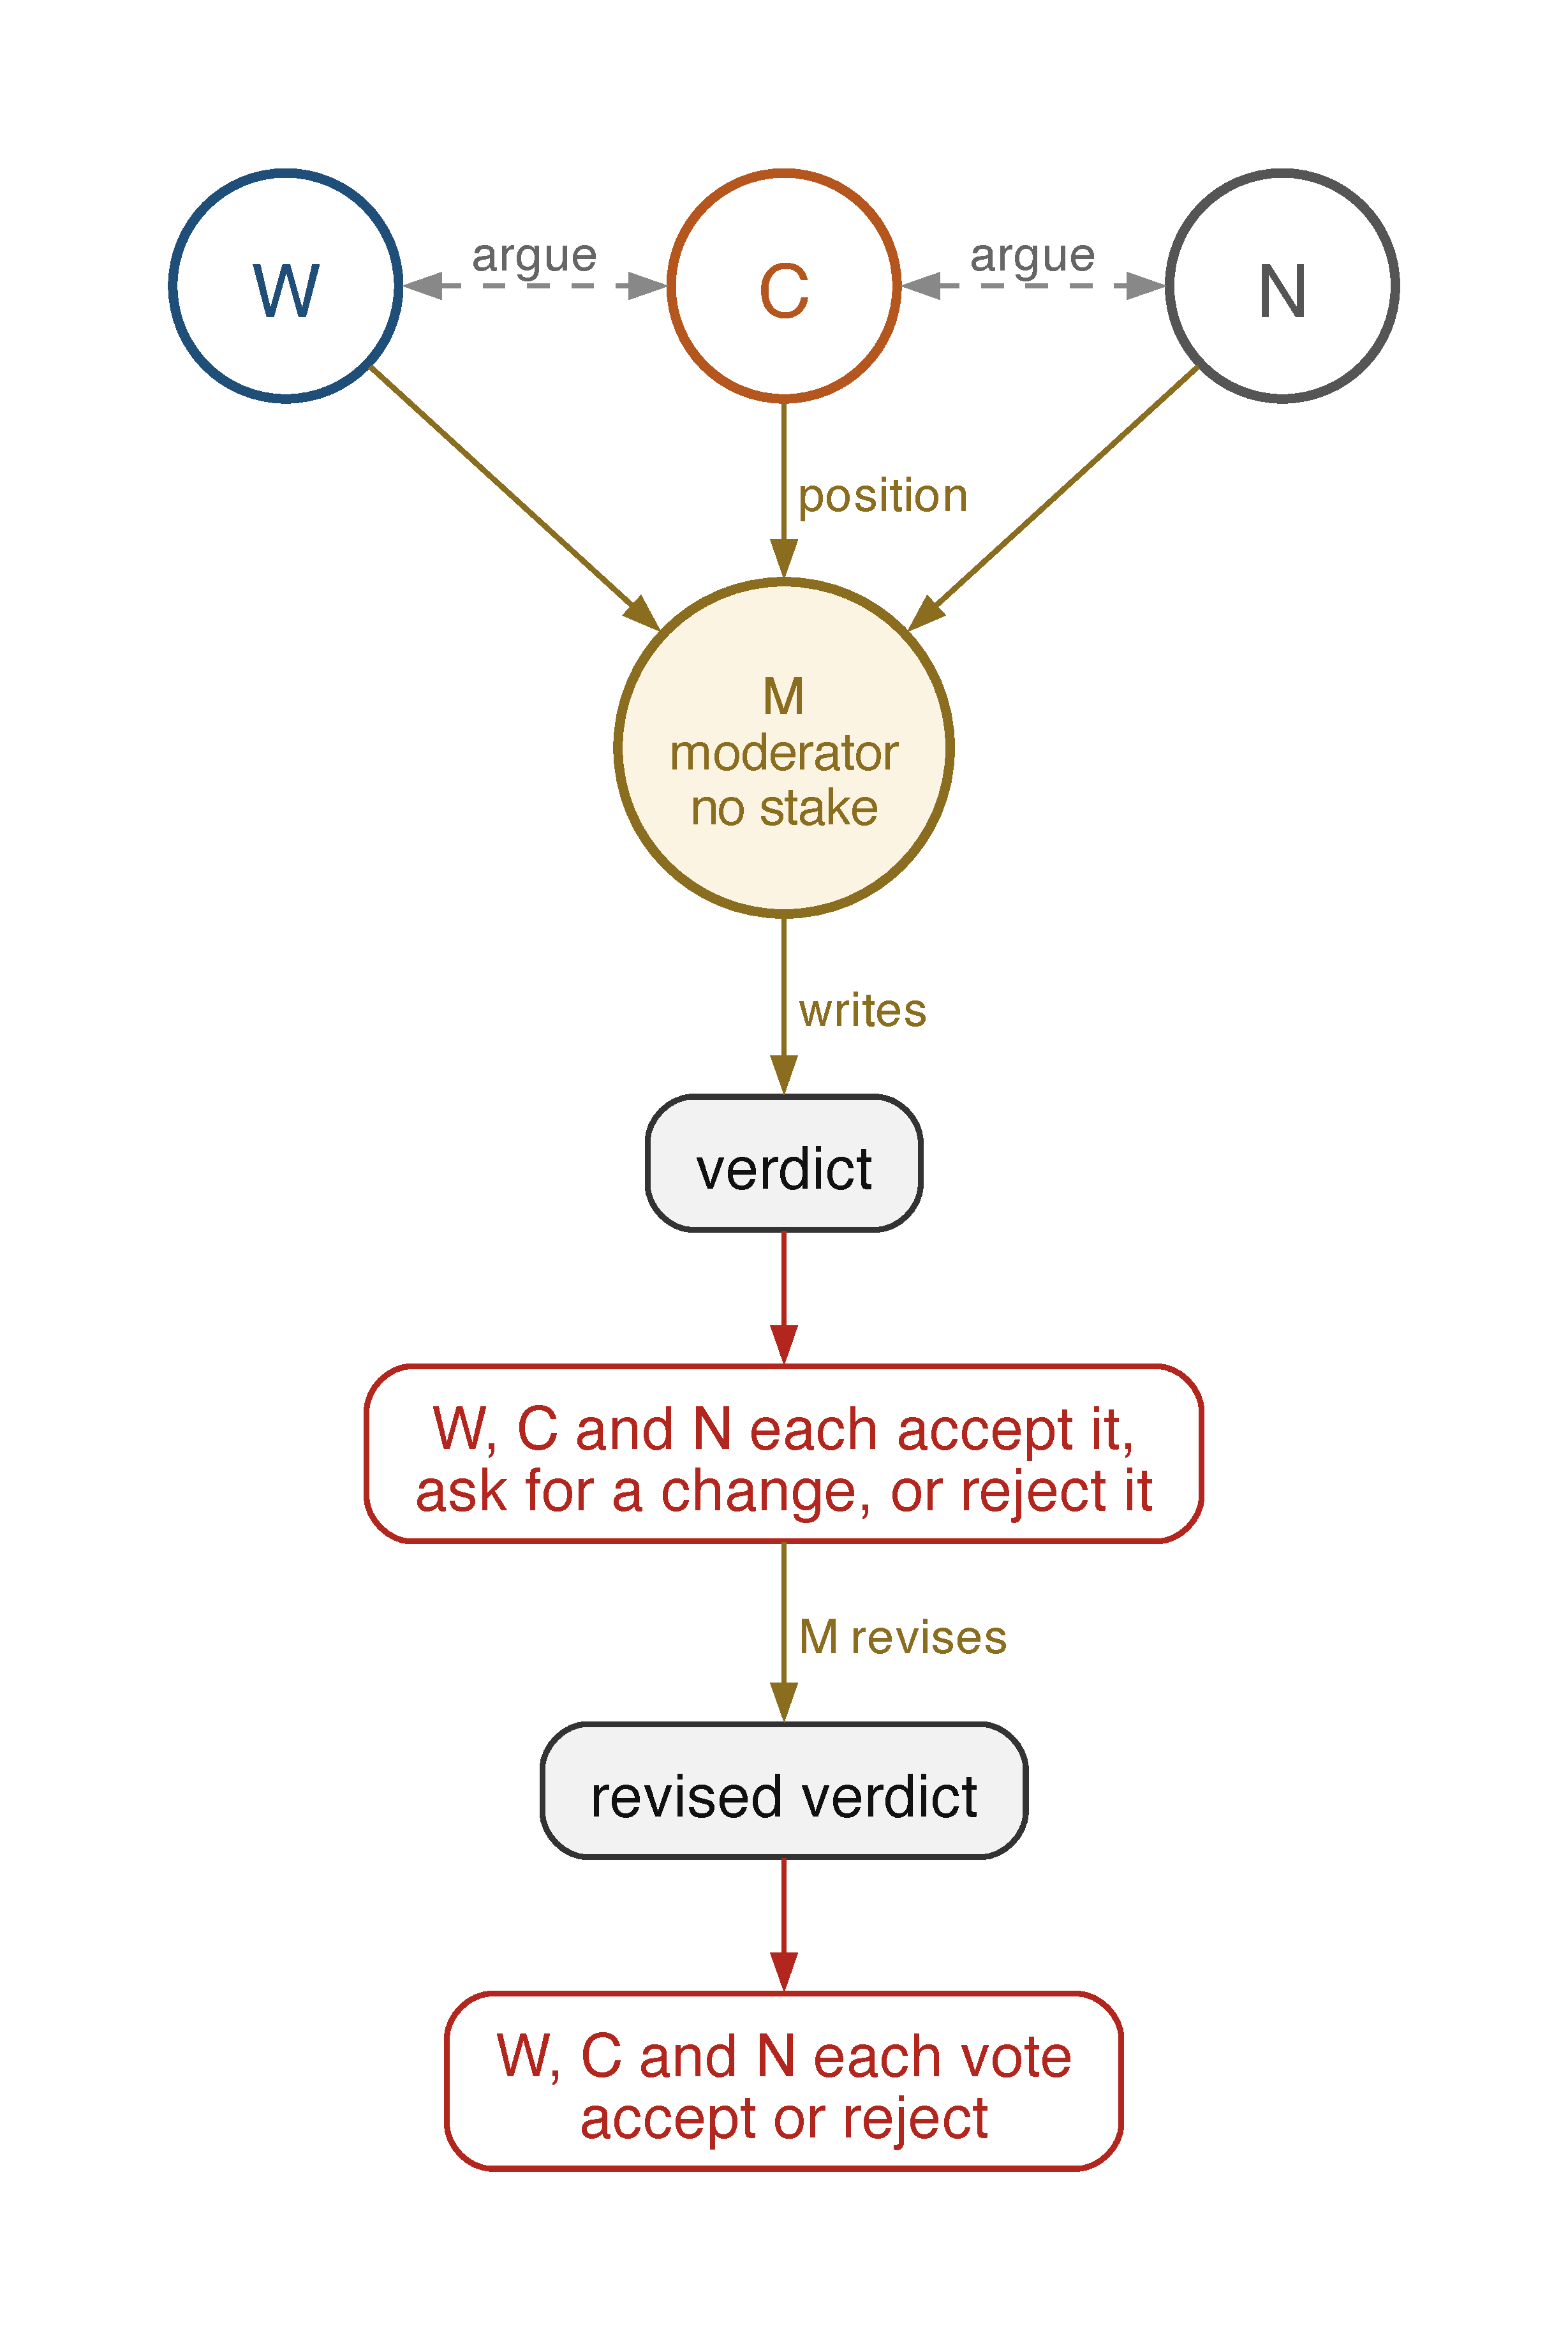
\includegraphics[width=\linewidth]{figures/fig_mechanism_b.pdf}%
\end{minipage}
\caption{(A) Three copies of one model read one account, briefed for the
writer, the other party or no one. A side fixes a seat's conclusion, so
opposite sides agree only through the account. (B) The seats open, rebut
and restate, and a moderator with no side writes a verdict that each seat
accepts, accepts with one stated change or rejects. (C) The losing party's
seat is expected to object. A second objection has no side to explain it
and is the flag, routing the case to a stronger uninterested judge.}
\label{fig-mechanism}
\end{figure}

\subsection{Embodiment as a control}
\label{sec-method-embodiment}
\label{sec-method-interventions}

A seat is a copy of one model reading the account under a brief that
names whom it speaks for and what it wants
(Figure~\ref{fig-mechanism}A). % code run_crowdgold_deliberation.py:461-511 (ROLES, the three briefs), 668-672 (the brief in the user turn under the narration system prompt)
We chose a side over a persona because a persona changes how a copy
speaks and a side fixes what it concludes, which makes it a control.
Told it speaks for the writer, a copy finds the writer not at fault on
99.7 percent of opening statements, and for the other party, at fault on
97.4
percent. % prereg L4160 (16.10 RESULTS, per-seat P(at_fault) at r0, 0.003 / 0.974 / 0.430), L5251 (16.16 RESULTS, the same), L3276-3277 (role-lock defined on these rates); design 2(a)
Two seats hold opposite sides because what two locked seats agree on
came from neither brief and must come from the account
\citep{milgrom1986relying,dewatripont1999advocates}. % design 2(a)
A third seat has no side because the verdict layer needs one uninterested
reader, and where the sides lock it is the seat any vote returns and the
best seat (Section~\ref{sec-results}). % design 2(b), 2(g); prereg L4494-4496 (16.15.4 RESULTS, majority equals the neutral seat on 1,642 of 1,642 debates, best seat neutral, reported in results.tex)
Neither advocate may invent facts, and the writer's seat may not assert
that the writer is not in the wrong where the account does not support
it, so no objection can rest on what the account lacks. Provability need
only be partial, since a decider who knows the speakers' interests
conflict can count on one to correct a mistaken inference
\citep{lipman1995robust}. % code run_crowdgold_deliberation.py:466-476 (writer's seat: may not invent facts, may not assert the writer is not in the wrong if the account does not support it), 483-493 (other party's seat: may not invent facts, at 492-493); the neutral brief (496-510) carries neither clause; design 3 (the flag must come from the account)
Every seat narrates before it commits, the light dose, under the model's
own scaffold so arrangement is the only
difference. % code run_phase1_quartet.py:102-116 (PROMPTS["narrative_cot"], the seats' system prompt, five first-person parts, who decides, who has a stake, what each action does to them, what stays uncertain, then a decision, as introduction_clean.tex L23-27 states); run_crowdgold_deliberation.py:544-556 (the comment stating why the scaffold is not written in the runner), 557-570 (agent_system pulls the live PROMPTS entry)
Removing it later showed it amplifies a second seat's objection without
creating the pattern. % prereg L5194-5215 (16.16 registration), L5261-5269 (16.16 pre-declared reading, narration not load-bearing for lock, localisation or concentration, part of what makes an advocate object against its side); design 2(e); readouts in results.tex
The writer's brief treats a finding against the writer as a finding
against its party and puts the case as strongly as the account allows. The
other party's brief treats a finding for the writer as a finding against
its party, one that did not write the account and cannot add to it, and
puts that case as strongly as the writer's own account allows. The
neutral brief speaks for everyone who will read the verdict and wants only
the finding the account supports. % code run_crowdgold_deliberation.py:466-476 (writer, stake not_at_fault), 483-493 (other party, stake at_fault, "a finding that the writer is not in the wrong is ... a finding against the party you speak for"), 496-510 (neutral, stake none); the three briefs paraphrased one sentence each

\subsection{The collective as a graph}
\label{sec-method-collective}

An arrangement of seats is a graph, its nodes the seats and a moderator,
its edges who reads whom (Figure~\ref{fig-mechanism}B), three copies of
one model running seven stages in seventeen
calls. % code run_crowdgold_deliberation.py:12-28, 889-904 (ROUNDS, CALLS_PER_CELL 17); artefact emergent_graphs.json protocol.stages
Each seat opens alone with a position and a verdict, so lock is measured
first. % code run_crowdgold_deliberation.py:685-697 (r0_user, the account and the brief only)
Each then rebuts the other two and restates a final position, the only
stages where seats read one another, six edges the no-edge control
cuts. % code run_crowdgold_deliberation.py:720-751 (r1_user, r2_user); prereg L3508-3516; artefact emergent_graphs.json protocol.edges (six read arcs at r1 and r2)
A moderator, a separate node with no stake, reads the account and the
three final positions and writes one synthesis and verdict, separating
arguing from
deciding. % code run_crowdgold_deliberation.py:576-586 (SYNTHESIS_SYSTEM), 753-770 (synthesis_user)
It is the seats' model by default, so the collective adds only an
arrangement, and was varied later because nothing in the design fixes who
decides. % code run_crowdgold_deliberation.py:1070, 3297-3299 (--moderator-model defaults to the agent model); prereg L5309-5345 (16.17 registration); design 2(d), 2(g)
At the objection round each seat accepts the synthesis, accepts it with
one stated modification, or rejects it naming the concern no integration
could
absorb. % code run_crowdgold_deliberation.py:786-818 (r3_label_user, the synthesis shown beside the seat's own final position, the modification one sentence on a marked line); 400-402 (MOD_MARKER, UNRESOLVABLE_MARKER)
A stated change is required because the synthesis is the first concrete
proposal there is to change, because integration must answer something,
and because a seat that accepts once its own change is addressed has
revised rather than opined. An objection without one is a counted
parse
failure. % code run_crowdgold_deliberation.py:788-793 (r3_label_user docstring, the first moment there is a concrete proposal to modify, what makes an R4 acceptance a revision rather than a first opinion), 856-862 (r4_vote_user docstring, own label and request quoted back, without them an acceptance is an opinion, not a revision), 587-597 (INTEGRATION_SYSTEM, says whose request each part answers), 634-647 (extract_objection, an empty statement with a non-ACCEPT label is a parse failure, counted and guarded), 1227 (objection_unstated)
The moderator then integrates, saying whose request each part answers,
and each seat votes accept or
reject. % code run_crowdgold_deliberation.py:587-597 (INTEGRATION_SYSTEM), 820-885 (integration_user, r4_vote_user)
% Labels, requests and votes are parsed from line-anchored markers, never by a judge model:
% code run_crowdgold_deliberation.py:400-402, 616-660 (marker_line, extract_objection,
% extract_addressed; a missing marker is a counted parse failure, never read as acceptance).
% The forced verdict line is stated with the verdict collapse in sec-method-instruments.

A moderator decides rather than a vote because where the sides lock a
vote adds nothing. Two fixed opposite verdicts cancel, so the majority is
the neutral seat's verdict, any weighting
\citep{shapley1984optimizing} can only reweight two constants, and three
draws of one model lack the independent errors a jury theorem needs
\citep{ladha1992condorcet}. % design 2(b) (the naive decider; the fitted weighted rule in aggregation_rules.json is unregistered and stays out of Methods), 2(d), 2(g); prereg L4494-4496 (16.15.4 RESULTS, majority equals the neutral seat on 1,642 of 1,642 debates where lock holds, reported in results.tex); the weighting clause is analytic, two locked seats are constants whatever their weights
The moderator is instead the node whose verdict the seats criticise
\citep{mercier2011argumentative,longino1990science}, sitting off the
argument because a network converges only when no node dominates it
\citep{golub2010naive}. % design 2(d) (the moderator earns its place as the node whose labels create the objection round), 6 (a hierarchy makes the root dominant); introduction_clean.tex L42-53 (the same framing)
Across cells the item text, verdict instruction and briefs are
byte-identical except for what a control varies, so cells differ only in
arrangement. % code verdict_format.py:263-280; run_stance_factorial.py:362-396; run_crowdgold_deliberation.py:458-460 (briefs arm-invariant, asserted at import); run_crowdgold_aita.py:197-230 (two framings over identical post text); prereg L3525-3532 (16.10, verdict instruction byte-identical), L5320-5322 (16.17, briefs verbatim), L5729-5737 (16.19, briefs verbatim)
% Token caps: 2,560 seat, 1,024 moderator, 1,024 label, 512 vote, raised to 3,072 for the two
% Anthropic models after the guard failure (prereg L3292, L1240-1252; code
% run_crowdgold_deliberation.py:1043-1046, 3306-3317); gpt-5.4-nano ran at a floor of 8,192
% on every call (generators.py:624, eff_tokens = max(max_tokens, 8192) for reasoning models).

\subsection{The flag}
\label{sec-method-flag}

Suppose the verdict goes against one party (Figure~\ref{fig-mechanism}C).
Only that party's seat has reason to object, and that expected objection
says nothing about whether the verdict is right. A second objection comes
from the seat whose side won or the seat with none. No brief put it there,
so it must come from the account, and an admission against interest is
what a listener who knows only the interests can trust
\citep{milgrom1986relying,lipman1995robust}. % design section 3 (the credible-signal principle)
On one-loser verdicts exactly one seat objects on 92 percent of debates,
two or more on 7
percent. % prereg L3664-3666 (16.12 table, one-loser stratum, 1,288 debates, P(exactly 1) 0.922, P(2+) 0.072)
As implemented the flag is a stake-blind count, firing when at least two
of the three seats, the uninterested seat included, object at the
objection round. % code run_crowdgold_deliberation.py:1205 (objected = label in ACCEPT_WITH_MODIFICATION, REJECT), 1298 (n_objectors); analyze_router_decomposition.py:148-149; prereg L3902 (the registered sensor is the n_objectors >= 2 counter); design section 1 (protocol.edges[15] spans W, C and N; the one-loser split of firings between the two cases is a result and sits in results.tex)
An earlier stake-aware composite, firing on the neutral seat's objection
or an advocate's against interest, needs each seat's stake and the
verdict's direction, which the plain count matches without
either. % prereg L3044-3069 (16.1 check 1, the counter is nested in the composite, composed accuracy 0.8801 against 0.8813, paired difference +0.0012; the counts are a result and stay in results.tex); code analyze_loop_step.py:88-111 (mislocalised, neutral_objected, flagged); analyze_claim_audit.py:70-71 (n_objectors_ge2)
Because the flag marks debates most likely to be wrong, a stronger
uninterested judge is paid for only there, answering flagged cases cold
by majority of three samples, ties to the
collective. % the deployed rule emits the collective's verdict unless the flag fired and the judge's majority otherwise; code analyze_claim_audit.py:103-107 (composed_ok); analyze_actuator_ladder.py:152-175; prereg L2492-2497 (the judge is the registration's actuator), L3914-3917 (the deployed rule)
The flag needs a verdict with one loser, a hypothesis about the verdict
rather than the model, and fails by design in three settings. A verdict
blaming both parties or neither gives both sides reason to object and it
floods. Seats that never leave their sides give no second objection and
it is silent. A plan every party gains from has no loser and nothing to
read. % design section 3 (flooding, silence, no counterparty); prereg L3653 (16.12), L2594 (Dilemmas, 6 of 624), L4753 (binding games, no objection on any debate); readouts in results.tex sec-results-extent

\subsection{Controls that isolate each decision}
\label{sec-method-controls}
\label{sec-method-designs}

Each decision was tested by removing or varying it, everything else held
at the registered protocol, further departures disclosed in the record,
outcomes in
Section~\ref{sec-results}. % prereg L3508-3510 ("everything else held at the registered protocol"), L3508-3523 (16.10, each cell in its own cache namespace, one sample per item and framing, 420 debates per cell beside the 1,680-debate embodied panel), L4136; code run_crowdgold_topology.py:86-100; artefact topology_2x2_analysis.json cells.*.n_debates (1680 / 420 / 420 / 420)
To test whether the stake is load-bearing we cut the first-person
alignment and the stake clause from every brief and the preamble, keeping
the instruction to argue as strongly as the account allows. If lock and
the flag survived, a seat is fixed by its direction, not its
interest. % prereg L3300-3310 (16.8 registration, the control is not confounded with an instruction to stop arguing; L3306-3309, disclosed departures: the three seat labels and the stake framing in the R0 preamble and both moderator system prompts); code run_crowdgold_unembodied.py:97-160 (the stake-free briefs, role ids reader_writer_situation, reader_other_situation, reader_norm) and 179-200 (preamble and moderator prompts)
To test whether opposed sides are load-bearing we made the roles
identical, three copies of the neutral brief. If the flag survived, it
belongs to three readers, not
opposition. % prereg L3508-3516 (16.10 registration, identical cells); code run_crowdgold_topology.py:45-61
To test whether the exchange is load-bearing we cut the edges, each seat
developing its own opening instead of rebutting. If the flag survived, it
belongs to the sides, not the
conversation. % prereg L3525-3532 (no seat reads any other; persuasion clause and verdict instruction byte-identical); code run_crowdgold_topology.py:50-61, 116-127
% Pre-declared readings (prereg L3560-3570): structure present with edges cut and absent
% under identical roles is H-ROLE, the reverse H-EDGE; stated in results.tex, not here.
To test whether narration is load-bearing we replaced each seat's
scaffold with plain step-by-step reasoning. If the flag
survived, narration is manner, not
mechanism. % prereg L5194-5215 (16.16 registration, PROMPTS["standard_cot"] in place of the scaffold, briefs and moderator unchanged); code run_crowdgold_deliberation.py:557-570 (agent_system standard_cot); run_phase1_quartet.py:77-79
To test whether the decider's model matters we put another vendor's
moderator over the same seats, their opening, rebuttal and restatement
replayed from cache and their labels and votes written afresh. If the
verdict did not move, the moderator counts verdicts rather than reading
arguments. % prereg L5309-5345 (16.17 registration, sonnet and haiku moderators; L5333-5343, r0 to r2 for the three seats replay from the registered cache, synthesis, integration, r3_label x3 and r4_vote x3 new, 3,780 replays and 3,360 new generations per cell; the moderator prompts differ from the registered ones by nothing but the moderator string); code run_crowdgold_modvendor.py
To test whether a second seat on the same side adds anything we seated a
like-biased ally beside the writer's under a mirrored brief. If it added
dissent, number rather than opposition carries the information
\citep{krishna2001model}. % prereg L5720-5750 (16.19 registration, four seats, the ally brief mirrors the writer brief sentence for sentence, other briefs verbatim, 22 calls per debate); code run_crowdgold_coalition.py; design 2(a)
To test whether the one-loser condition is a limit or an artefact of two
advocates we seated an advocate for a third person the account names, so a
verdict could have two losers. If the flag kept its meaning, the
condition is an
artefact. % prereg L6100-6150 (16.21 registration, screen for a named third party, k in {1, 2}), L6183-6184 (at k = 2 the stake-blind count fires by construction and only the against-interest count is informative), L6126-6140 (disclosed departures, a screened 143-item panel and a new brief); code run_crowdgold_nperspective.py, screen_third_party.py; design 3, 4
To test whether same-model seats limit the verdict we served the three
identical no-edge seats from three vendors. If they aggregated no better
than three copies, shared errors are not the limit
\citep{ladha1992condorcet}. % prereg L5539-5580 (16.18 registration, seats haiku, nano and grok, no edges, grok moderator, no vendor name in any prompt, 197 items, 394 debates); code run_crowdgold_multivendor.py; design 2(g)
To test whether repetition alone deepens a perspective, one agent re-read
and re-answered its own false-premise answer, against a control fed its
untreated one. If it did, the collective would be mere
iteration. % prereg L3724-3742, L3769-3779 (16.14 registration, gpt-5.4-nano, prior fed back in full under a shared bridge byte-identical across arms, readout a difference in differences of within-unit changes in affirmation), L3871-3886 (16.14b, 16,384 tokens after the 8,192 run exhausted completions, L3817-3833 GUARD FLAGGED), L4091-4097 (16.14b GUARD OK, the run read); code run_bm_cycle.py:78-136, 228-258; artefact bm_cycleb_analysis.json

\subsection{Instruments, measures and estimation}
\label{sec-method-instruments}
\label{sec-method-measures}
\label{sec-method-estimation}

Disputes (Table~\ref{tab-instruments}) are Scruples Anecdotes,
first-person conflict accounts whose crowd verdict is gold when at least
90 percent of at least 50 votes agree, 249 items under two framings, 210
after one model's
refusals.
\todo{references.bib Scruples entry, Lourie, Le Bras and Choi 2021, PI to add} % code load_scruples.py:10-13 (five verdict classes), 131-132, 356-359, 771-786 (the plurality class); artefact crowdgold_aita_summary.json:7-11 (99 at fault, 150 not); code run_crowdgold_aita.py:197-230 (the two framings, as someone else's account and as the asker's own, over identical post text), artefact crowdgold_aita_summary.json wrapper_match; screen = items a model's cached single-agent call refused, dropped for that model, code run_crowdgold_deliberation.py:2092-2129, prereg L528-531, L534-536 (E5 RESULTS), 220 for the pilot at prereg L396-397 and cg_delib_pilot_console.log:40. NOTE for the PI: E5 RESULTS L534-536 says 219 -> 210 against 220 in E4 and the console log; reconcile the record.
False premises are 100 BrokenMath \citep{petrov2025brokenmath} problems
with a false statement, six samples per item
on gpt-5.4-nano \citep{openai_gpt54nano}, under heads making the model
the statement's author, a colleague, a stranger or a
rival. % code load_brokenmath.py:4-5 (sampled from the 451 false-statement problems, every gold FALSE); run_stance_factorial.py:189-199 (fixed prefix), 438-441 (seed 44); run_bm_embodiment.py:60-67, 83-104, 138-155; prereg L50-56 (one-sentence heads token-matched within a ratio of 1.10, none claiming to know whether it is true), L34-37, L42-48 (2,048 tokens), L227-238 and code run_bm_cross_sig.py:72-86 (three arms crossing the heads with narration); analyze_bm_embodiment.py:27-31, 70-97 (all 600 units in the denominator, an empty response counting as no verdict)
Dilemmas pair two anecdotes, a fresh crowd naming the worse action,
ELEPHANT \citep{cheng25elephant} supplies 150 personal questions judged
for validation of the asker, and 144 ordinal two-by-two games with a
first-principles gold plan ran binding, non-binding, and as coordination
on nine two-equilibrium
games. % Dilemmas seat an advocate for each person and a neutral seat; prereg L2285-2302, L2314-2319, L2331-2340, L2366-2369 (one framing, neither account addressed to the model); code load_scruples_dilemmas.py:16-27; run_crowdgold_dilemma.py:121-136, 229-312; ELEPHANT answered under the untreated prompt and under narration, code run_elephant.py:376 (n 150), rescore_elephant_untruncated.py:112; elephant_scorers.py:20-48, 174-193 (the benchmark's own judge prompt, claude-haiku-4-5, binary score); artefact length_matched_elephant_oeq_validation_corrected.json
% Truncation artefact: the judge pipeline cut answers at 4,000 characters, most narrated
% answers affected, every affected answer re-scored on its full text (elephant_scorers.py:193;
% rescore_elephant_untruncated.py:1-30, 65, 122-164); results.tex states the correction.
% Games: prereg L4034-4048 (16.13 instrument, masked leak gate), L4719-4725, L4734-4736, L5018, L4793-4870 (16.13c, non-binding beside a solo comparator), L5060, L5108-5145 (16.13d), L5147, L5114-5117 and L5129-5131 (COORD scoring rule, a recommendation coordinates only when it names a pure equilibrium); code tmg_games.py, run_game_singleagent.py, run_crowdgold_game.py, run_crowdgold_game_nb.py, analyze_game_coordination.py (is_nash on the recommended cell); artefacts game_*_analysis.json; readouts in results.tex sec-results-extent
Dispute verdicts, parsed from a forced line and never by a judge model,
collapse to at fault (YTA, ESH) or not (NTA, NAH), dropping UNRESOLVED,
while on false premises UNRESOLVED is never correct and stays in the
denominator. % code verdict_format.py:380-449 (extract_verdict, forced VERDICT line, NOVERDICT on ambiguity), 32-34, 100-101; load_scruples.py:128-129; analyze_crowdgold_sdt.py:113-131

Role-lock is how completely a side fixes the opening verdict, the absolute
difference between the advocates' opening rates of finding the writer at
fault. % prereg L3276-3277; code analyze_topology_2x2.py:156-157 (lock = abs(p_at[W] - p_at[C]))
The fire rate is the share of debates on which the flag fires, over all
debates in the two-by-two readouts and over codable debates when read as
routing
coverage. % code analyze_unembodied_ablation.py:171-192 (fire_observed over all loaded rows, load_rows 88-117 keeps every debate and only tags codability), analyze_topology_2x2.py:129-130, 227 (loc["fire_observed"] written as objection.fire_rate; 329 of 1,680 raw debates = 0.196, prereg L4149-4151); analyze_router_decomposition.py:193-214 (coverage over codable debates, analyze_actuator_ladder.py:103-104 drops non-codable debates before build_cells)
Lift is the probability the integrated verdict is wrong given the flag
minus that given no flag, error concentration their ratio, both read
within verdict strata because the flag floods on both-party
verdicts. % prereg L594-595, L3900-3915 (16.15.1 registration, one loser for YTA or NTA and both parties for ESH or NAH), L4247-4268 (resampling frame, strata restricted inside each draw, the S2 verdict as stratum source), L4275 (lift and ratio columns); lift read on the integrated verdict for the counter and on the synthesis verdict for the earlier composite; code analyze_router_decomposition.py:139-146, 183-247; analyze_loop_step.py:205-214 (syn_ok); analyze_unembodied_ablation.py:204-215 (s2_ok); artefact router_decomposition.json counter_lift_by_stratum
Transfer is the same flag read against a model that never saw the debate,
answering alone by majority over three
samples. % a cell of item and framing is flagged when more than half of its debates flagged it, all debates in the two-by-two readouts (analyze_topology_2x2.py:193-198) and codable debates in the routing readouts (analyze_router_decomposition.py:322-347; analyze_actuator_ladder.py:103-104); prereg L3948-3955 (16.15.3), L3933-3946 (16.15.2, the solo's own free signals, a both-party verdict or sample disagreement, set against the flag on the same 420 cells); code analyze_unembodied_ablation.py:204-215; analyze_topology_2x2.py:18-19, 184-204; analyze_router_decomposition.py:322-347, 374-448; artefacts transfer_readouts.json, router_decomposition.json solo_signals
Composed accuracy is the deployed system's, with claude-haiku-4-5 or a
cached claude-sonnet-4-6 as
judge. % prereg L3914-3920, L4285-4326 (16.15.1, counter, verdict-type and union routers, against random routing at matched coverage over 200 seeds), L3584-3594, L3608-3612 (16.11a, a second design with base grok alone, judge sonnet, router the flag or its union with the base's own sample disagreement); code analyze_router_decomposition.py:97-101, 152-168, 251-263; analyze_claim_audit.py:60; artefact router_decomposition.json composed_haiku, composed_sonnet
% Carried for results.tex, definitions only. Effective voter count, stated only where the
% roles lock, read from how often the three-seat majority equals the neutral seat on debates
% with three codable opening verdicts, and from the oracle gap, a two-fold cross-validated
% lookup table over those verdicts minus the neutral seat, folds over items (prereg
% L3957-3967, L4462-4470, L4515-4529; code analyze_effective_voter.py:21-31, 177-247;
% artefact effective_voter.json). Localisation, the share of debates with exactly one
% objector minus the Poisson-binomial prediction from the seats' own objection rates (prereg
% L3251-3262; code analyze_unembodied_ablation.py:144-192). Grip, a fire rate of at most one
% half, final rejections of at least five percent, and stake-seat rejection at least 0.20
% higher when the integrated proposal undermines the seat's stake (prereg L1169-1181; code
% analyze_stake_grip.py:39, 151-179; run_crowdgold_deliberation.py:522-540, 1180-1204).
% Actuator-ladder bar, a gain positive when its interval excludes zero, its point is at least
% 0.05 and its sign replicates across item halves and framings (prereg L755-770; code
% analyze_actuator_ladder.py:53-64); the second design required only a gain over the base
% and over the judge used everywhere, each excluding zero (prereg L3592-3594).

Every interval is an item-clustered percentile bootstrap with 2,000 to
10,000 draws, families Bonferroni-corrected, missing false-premise units
Manski-bounded. % prereg L75-76, L541-542, L4226-4236, L762-765, L105-107; code analyze_actuator_ladder.py:55 (4,000), analyze_claim_audit.py:61, analyze_unembodied_ablation.py:68, analyze_topology_2x2.py:339 (3,000), analyze_stake_grip.py:57-68 (2,000), analyze_router_decomposition.py:97 and analyze_effective_voter.py:106 (4,000, seed 13), analyze_length_matched_elephant.py (8,000), run_bm_cycle.py:228 (4,000, seed 11); analyze_dilemma_sensor_search.py:111-116
Two guards run before any number is read, truncation and no legal verdict
each at most five percent per cell and call, failing runs going
unread. % code run_crowdgold_aita.py:972-999; run_crowdgold_deliberation.py:3532-3538, 3620-3623 (the literal string); prereg L1240-1252 (the first Anthropic runs retracted), L3639-3651 (the gpt-4o screen unread)
Controls pass a parse gate of at most 0.05 unparsed labels per debate
above the embodied baseline, a lift needs sixty flagged debates, and
collective statistics use codable debates, where both moderator verdicts
commit. % prereg L3335-3337 (mean n_r3_unparsed per debate must not exceed the embodied baseline by more than 0.05 seats), L2571-2574, L4226-4229; code analyze_unembodied_ablation.py:69-70 (PARSE_GATE_SLACK), 275-276 (gate_parse against baseline + slack), 111-113 (codable = synthesis and final verdict both code); analyze_dilemma_grip.py:62-66
One pre-registration document with dated addenda fixed hypotheses,
estimators, kill criteria, ceiling and stop rule before any call, results
appended, nothing above them edited, two overruns
reported. % prereg L3-4, L139, L296-303; L1297-1301 (Addendum 6, $70.47 against $40, "PI authorized the overrun explicitly"); L2566-2569, L2580-2589 (Addendum 12 Stage 2, ~$9.41 against $8, under the registered stop rule)
% Addenda map: E1 to E5 cover the false-premise and disputes experiments, 6 the grip screens,
% 12 and 13 the comparative instrument, 16 the claim audit and ablations (16.8, 16.10, 16.14,
% 16.15, 16.16), 16.17 to 16.21 the cross-vendor moderator, cross-vendor deciders, coalition
% and n-perspective cells. prereg L139, L331, L396, L528, L1169, L2366, L2716, L3033, L3237,
% L3504, L3704, L3888, L5194, L5309, L5539, L5720, L6100.

\begin{table}[t]
\centering
\footnotesize
\caption{Instruments. Item counts are the panels the reported statistics
use. Models by vendor card
\citep{xai_grok41,anthropic_haiku45,anthropic_sonnet46,openai_gpt54nano}.}
\label{tab-instruments}
\setlength{\tabcolsep}{4pt}
\begin{tabular}{p{2.1cm}p{2.3cm}p{2.7cm}p{2.9cm}p{2.1cm}}
\toprule
Instrument & Items & Gold & Verdict set & Models \\
\midrule
Disputes (AITA) & 249 panel, 210 deliberated % artefact crowdgold_aita_summary.json:7-11; prereg L528-531
  & crowd plurality, $\geq 90\%$ of $\geq 50$ votes % code load_scruples.py:131-132
  & YTA, NTA, ESH, NAH, UNRESOLVED % code verdict_format.py:101
  & grok, haiku, sonnet, nano \\ % prereg L1307-1310, L3608
False premise (BrokenMath) & 100, all gold FALSE % code run_bm_embodiment.py:61-62; run_stance_factorial.py:438-441
  & benchmark, false stratum % code load_brokenmath.py:4-5
  & TRUE, FALSE, UNRESOLVED % code verdict_format.py:100
  & nano \\ % code run_bm_embodiment.py:60
Comparative (Dilemmas) & 80 then 700, 624 codable % prereg L2370-2373, L2566-2574
  & fresh crowd, $\geq 4$ annotators % prereg L2314-2319
  & ACTION\_A, ACTION\_B, UNRESOLVED % code run_crowdgold_dilemma.py:121-136, 304-312
  & grok, haiku as judge \\ % prereg L2370, L2492-2497
Open-ended (ELEPHANT) & 150 per generator % artefact length_matched_elephant_oeq_validation_corrected.json (cot_n 150)
  & none, judge-scored validation % code elephant_scorers.py:20-48
  & validates, does not % code elephant_scorers.py:165-172 (binary parse)
  & grok, haiku, sonnet, nano \\ % artefact length_matched_elephant_oeq_validation_corrected.json generators
Games (TMGBench) & 144, regions 16 / 97 / 31, nine two-equilibrium % prereg L4036-4038 (16.13 instrument, regions value 16 / neutral 97 / cannot-assist 31), L5110-5113 (16.13d registration, the nine CONFLICT_OF_EQUILIBRIA games)
  & first-principles plan % prereg L4036-4037 (gold reproduces the canonical file on 144 of 144), L4822-4827 (non-binding gold)
  & PLAN\_xy, NO\_UNIQUE\_PLAN or NO\_RECOMMENDATION % prereg L4047-4048 (binding verdict set), L4814-4818 (non-binding: advocates ACT\_1 / ACT\_2, third seat and group PLAN\_xy / NO\_RECOMMENDATION)
  & grok \\ % prereg L4055 (Stage A, grok-4-1-fast-reasoning), L4719 (16.13 RESULTS), L5060, L5147
\bottomrule
\end{tabular}
\end{table}
